\documentclass[a4paper,10pt]{scrartcl}

\usepackage[utf8]{inputenc}
\usepackage[ngerman]{babel}
\usepackage[T1]{fontenc}
\usepackage{amsmath}
\usepackage[section]{placeins}
\usepackage{graphicx}
\usepackage{esvect}



\title{Praktikum B Vorbereitung zu Versuch "lb"}
\author{Leon Machtl und Raphael Lehner}
\date{05.02.2020}

\begin{document}
	\maketitle
	\tableofcontents
	\newpage
	
	\section{Einleitung zum Versuch}
	Inhaltlich fertig - Bilder fehlen noch und paar Formartierungen, aber ich hab immerhin was gemacht.-------------
	Die Beugung oder Diffraktion ist die Ablenkung von Wellen an einem Hindernis. Durch Beugung kann sich eine Welle in Raumbereiche ausbreiten, die auf geradem Weg durch das Hindernis versperrt wären. Jede Art von physikalischen Wellen kann Beugung zeigen. Besonders deutlich erkennbar ist sie bei Wasserwellen oder bei Schall. Bei Licht ist die Beugung ein Faktor, der das Auflösungsvermögen von Kamera-Objektiven und Teleskopen begrenzt. Manche technische Komponenten, wie Beugungsgitter, nutzen die Beugung gezielt aus. Zur Beugung kommt es durch Entstehung neuer Wellen entlang einer Wellenfront gemäß dem huygens-fresnelschen Prinzip. Es besagt, dass jeder Punkt einer Wellenfront als Ausgangspunkt einer neuen Welle, der so genannten Elementarwelle, betrachtet werden kann. Die neue Lage der Wellenfront ergibt sich durch Superposition sämtlicher Elementarwellen. Da die Elementarwelle eine Kugelform bzw. Kreisform hat,bildet sich auch eine rücklaufende Welle. Im Falle sehr enger Spalte bilden sich keine Wellenfronten mehr, da näherungsweise nur mehr eine einzige Elementarwelle den Spalt passieren kann. Hieraus ergeben sich eine Reihe von besonderen Eigenschaften, wie etwa das Entstehen von Interferrenzmustern. Für die folgenden Ausführungen wird i.d.R.von koheräntem und monochromatischen Licht ausgegangen, also von fester Phasenbeziehung und gleicher Wellenlänge aller beteiligten Photonen.
		
		\FloatBarrier
			\begin{figure}[h]
\centering
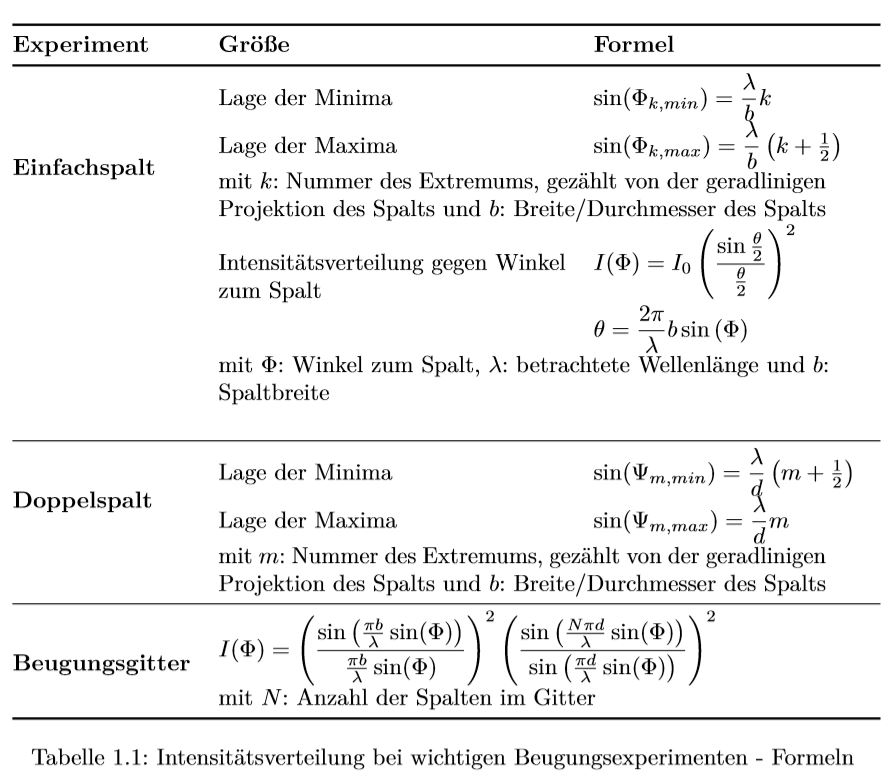
\includegraphics[width=0.9\textwidth]{./Bilder/lb01}

\end{figure}
\FloatBarrier
	\section{Fragen zur Vorbereitung}
		\subsection{Frage 1}
		Wie in Tabelle 1.1 aufgeführt ist die Lage der Extrema sowohl beim Einfach- als auch beim Doppelspalt abhängig von der Wellenlänge des durchfallenden Lichts. Die Wellenlänge ändert sich jedoch beim Übergang von einem Medium mit Brechungsindex n1 in eines mit Brechungsindex n2 nach: λ0 = λn1 n2 Vergleichen wir die Situation in Luft gegen die in Wasser, so gilt: nLuft < nWasser =⇒ Wellenlänge wird kürzer =⇒ die Extrema rücken näher zusammen.

		\subsection{Frage 2}
		DieÜberlagerungzweierEinzelspalt-Experimente ist qualitativ verschieden vom Ergebnis des Doppelspalt-Experiments. Im EinfachspaltExperiment treten keine Extrema II Klasse auf; das Bild des Doppelspalt-Experiments enthält dagegen solche Nebenextrema. Die Einhüllende des Doppelspalt-Bildes entspricht jedoch der Überlagerung zweier EinzelspaltBilder.

Bilder ...
		\subsection{Frage 3}
		Werden beide Spalte des Doppelspaltexperiments von zwei eigenständigen Laserlichtquellen belichtet, so erhält das Experiment folgende Freiheitsgrade:
		
		\FloatBarrier
			\begin{figure}[h]
\centering
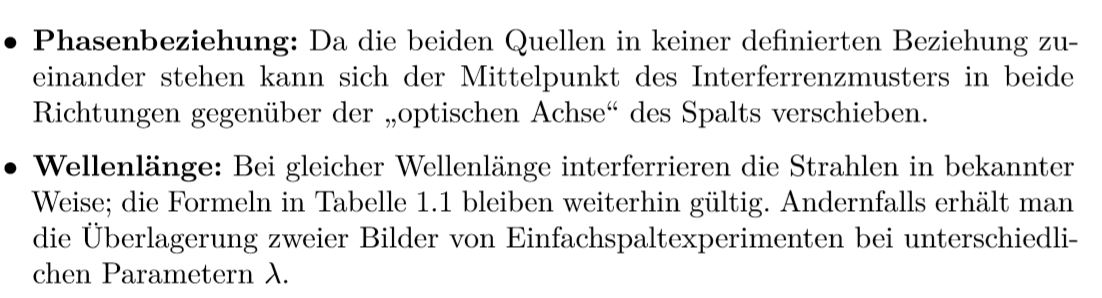
\includegraphics[width=0.9\textwidth]{./Bilder/lb02}

\end{figure}
\FloatBarrier

		\subsection{Frage 4}
		Stammt das Licht, das auf den Doppelspalt fällt, aus einer einzigen Lichtquelle, die mittels eines Strahlteilers auf beide Spalte gelenkt wird, so ist die Wellenlänge des einfallenden Lichts an beiden Spalten dieselbe. Jedoch hat das Licht unterschiedliche Laufzeiten und wird bei der Reflexion Phasenverschoben. Wie schon in der vorigen Aufgabe ist das Ergebnis eine (nicht definierte) Verschiebung des Interferrenzbildes gegenüber der Systemachse.

		\subsection{Frage 5}
		Quecksilberdampflampen emittieren (näherungsweise) ein Linienspektrum mit mehreren Peaks. Für jede der Anregungslinien entsteht ein eigenes Interferrenzmuster, die sich additiv überlagern. Aufgrund der menschlichen Wahrnehmung des Lichts (drei Arten farbempfindliche Sensorzellen) erscheint das Interferrenzmuster „regenbogenfarbig“.

Bilder ...
		\subsection{Frage 6}
		Bei der Entstehung der Interferrenzmuster ist es von Bedeutung,obdasaufdenSpaltfallendeLichtalsParallelstrahleneinfiel,oderobeinekomplexereBeziehung zwischen den Teilstrahlen bestand.
Man spricht von Fraunhoferbeugung, wenn der Spalt so belichtet wird, dass parallele Strahlen einfallen. Dies wird z.B.in guter Näherung durch eine Punktlichtquelle im Fernfeld des Spalts erreicht. Bei der Fresnelbeugung dagegen stand die Punktlichtquelle im Nahfeld des Spalts. In diesem Fall ist der Winkel, den die Strahlen zur optischen Achse (Lichtquelle – Spalt) einschließen nicht vernachlässigbar.

Bilder ...
			
							 			\subsection{Frage 7}
Ein Lichtstrahl, der durch einen Spalt der Breite b tritt wird gedanklich in N einzelne Strahlen im Abstand q =b/N zueinandereingeteilt.Nachdemhuygensfresnelschen Prinzip entstehen hinter dem Spalt nicht nur geradlinige Strahlen, sondern auch Strahlen, die in jede Richtung ϕ von der geraden Linie abweichen. Wenn diese auf einen geraden Schirm im Abstand d treffen,sohabensiezueinandereinenAbstand∆x und einen Gangunterschied von ∆s bzw. eine Phasendifferenz ∆ϕ. Es gilt:

	\FloatBarrier
			\begin{figure}[h]
\centering
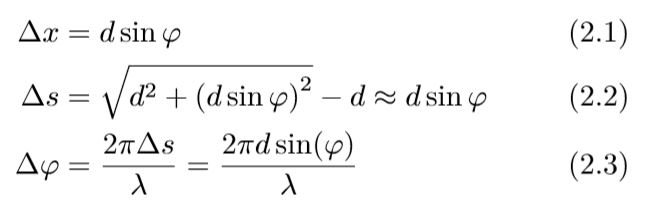
\includegraphics[width=0.6\textwidth]{./Bilder/lb03}

\end{figure}
\FloatBarrier
Jeder Strahl ist gegen seinen Nachbarn um ∆ϕ verschoben. Insgesamt überlagern sich also N Wellen mit der Amplitude A, die jeweils um ∆ϕ gegeneinander phasenversetzt schwingen. Das gesamte ~ E-Feld in einem festen Punkt wird also beschrieben durch:

\FloatBarrier
			\begin{figure}[h]
\centering
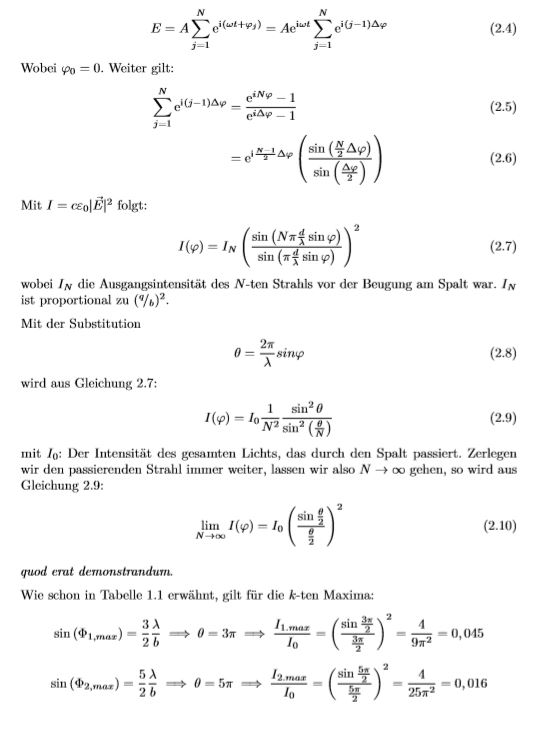
\includegraphics[width=0.9\textwidth]{./Bilder/lb04}

\end{figure}
\FloatBarrier

		\subsection{Frage 8}
		\FloatBarrier
			\begin{figure}[h]
\centering
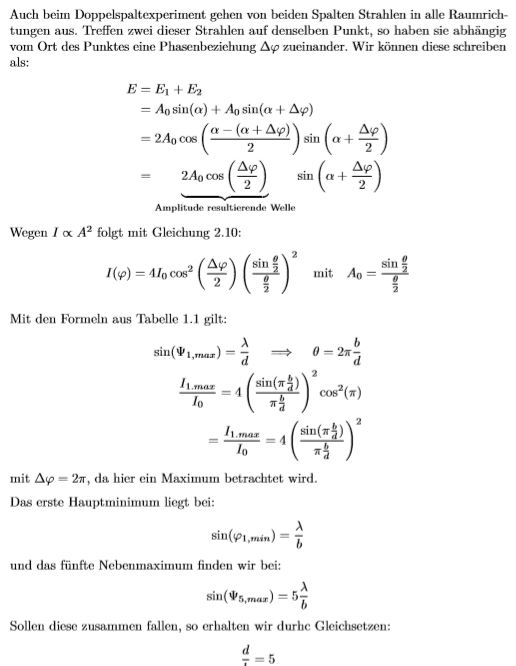
\includegraphics[width=0.85\textwidth]{./Bilder/lb05}

\end{figure}
\FloatBarrier

		
	\end{document}
